\subsection{Lineær bevægelse} \label{løsningsanal: Lineær bevægelse}
Det ønskes at finde en optimal bevægelsesform til flytning af PeJV under prikpåføring. Fra designspecifikationer kan det ses, at der lægges vægt på præcision og hastighed af prikplacering. Dette vil bruges til at vægte forskellige lineære løsningsforslag, og vurdere den bedste løsning.
Af disse grunde, vælges der at udelukke løsninger der er upræcise, langsomme og evt. for komplicerede til at være en optimal løsning. Dette efterlader valget mellem et tandremdrevet og et skruedrevet system. \parencite{IndustrialQuickSearch2025LinearPrinciples}

\textbf{Skruedrevet system} omfatter kugleskruer og ledeskruer. Ledeskruer omdanner roterende bevægelse til lineær bevægelse, gennem et gevind på skruen, hvortil genstanden der skal flyttes, sidder på skruen se figur \ref{fig:Ledeskrue - skitse}. Ved at bevæge gevindet vil genstanden bevæge sig med gevindets spiral og derved bevæge sig fremad.

Ledeskruer kræver færre dele og mindre vedligeholdelse end en kugleskrue. Tilgengæld er den mindre effektiv, grundet en større kontaktflade. Generelt gør ledeskruers simplere design, som ses i figur \ref{fig:Ledeskrue - skitse}, den billigere, hvor en kugleskrue kan have højere nøjagtighed og flytte tungere laster. Kugleskruers primære fordel er den lavere friktion og dermed højere effektivitet. Her er effektivitet et udtryk for forholdet mellem overført kraft og energi tabt til varme. (\cite{UniversalThreadGrindingCompany2020PrecisionAssemblies}; \cite{IndustrialQuickSearch2025LeadBenefits})

\begin{figure}[H]
    \centering
    \begin{subfigure}[b]{0.49\textwidth}
    \centering
        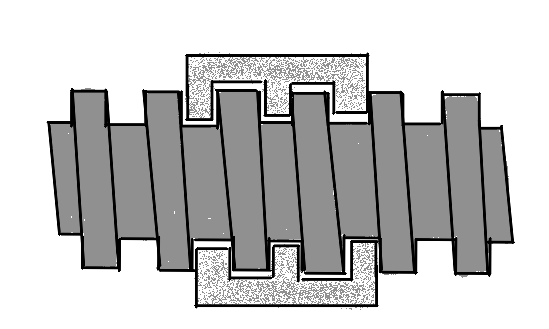
\includegraphics[width=\linewidth]{Sections/5 Konceptgenerering/Media/Ledeskrue-skitse.png}
      \caption{Skitse af ledeskrue}
       \label{fig:Ledeskrue - skitse} % Viljams mor når mig når(s)
  \end{subfigure}
    \hfill
  \begin{subfigure}[b]{0.49\textwidth}
    \centering
    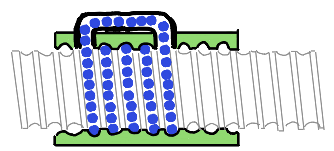
\includegraphics[width=\linewidth]{Sections/6 Detaljeløsning/Media/Ball nut.png}
    \caption{Kugleskrue illustration}
    \label{fig: Balls nut} % Mig når mig når når mig når viljams mor
  \end{subfigure}
    \caption{Skruedrevet systemer}
\end{figure} \plainbreak{-0.5}

Kugleskruer omsætter rotations kraft til lineære kraft, denne transformation opnås ved at rotere en skrue, hvorpå en kuglemøtrik er monteret. Kuglemøtriken indholder en mængde kugler, som bevæger sig i skurens gevind. Kuglernes bevægelse i gevindet resulterer i at kuglemøtriken skubbes langs skruen. Kuglemøtrikens udformning muliggør at kuglerne kan genanvendes, ved at når de kommer til enden føres de gennem kuglemøtriken tilbage til fronten af kuglerækken (Se figur \ref{fig: Balls nut}). Kugleskruer har en højere effektivitet end ledeskruer, da rullende kugler har en lavere friktions koeficient end to flader, der gnider mod hinanden, som i en ledeskrue. Kugleskruers afvigelse ligger lidt under $\SI{d-4}{mm/mm}$. (\cite{Jaffe2025PrecisionGround}; \cite{IndustrialQuickSearch2025BallBenefits})


\textbf{Tandremsdrevede systemer} er kendetegnet ved, at en motor roterer en tandremskive hvorpå en tandrem sidder. Denne tandrem er koblet til en genstand, der ønskes at bevæges langs bæltets længde. Når tandremmen roteres den ene vej, vil emnet blive trukket i den retning, og modsatte retning hvis rotationsvejen vendes. Det tandremsdrevede system, er effektivt under lange arbejdslængder, og kan opnå store hastigheder. Tandremmene har en risiko for at glide, samt består af mere elastiske materialer end skruerne, hvilket kan medføre en afvigelse i præcision. Tandremmes afvigelse ligger omkring \(\SI{d-3}{mm/mm}\) \parencite{Rollco2022BallWhat}. 

\begin{figure}[H]
    \centering
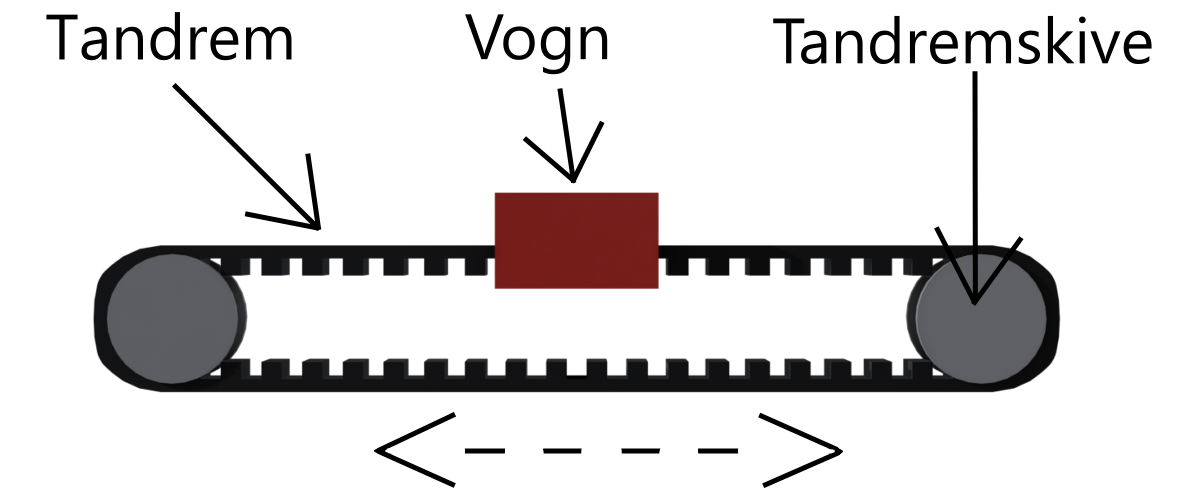
\includegraphics[width=0.65\linewidth]{Sections/5 Konceptgenerering/Media/Illustration af tandrem 7.png}
    \caption{Illustration af tandrem.}
    \label{fig: Illustration af tandrem}
\end{figure} \plainbreak{-.5}

Grundet materialerne tandremme er lavet af varierer, sammen med remmene bliver svage i løbet af deres levetid, betyder dette at præcisionen af tandremme afhænger af flere forskellige faktorer. For at tandremssystemer kan opnå den nødvendige præcision, kræver det mere justering og er mindre pålideligt over løsningens levetid. \parencite{Casillo2025Belt-DrivenInc} \\


\subsubsection{Valg af lineær bevægelse}  \plainbreak{-0.5}
Af forrige fremlagte muligheder, er kun ledeskruer og kugleskruer interessante, da der her skal fokuseres på korte afstande og stor præcision. Lede- og kugleskruer ligger begge mere end 1/5 under den maksimal acceptabel afvigelse på \(\SI{\pm0,1}{mm}\) over \(\SI{200}{mm}\), som er den største værdi i arbejdsområdets grænseværdi, hvilket gør begge brugbare.

Under prikplacering vil der ske mange accelerationer før arbejdsområdet er udfyldt, når der skiftes retninger. Dette betyder at en større acceleration vil gøre prikprocessen kortere. Accelerationen er en konsekvens af effektiviteten af skruen. Ledeskruer har typisk mellem 50\% og 70\% effektivitet, hvorimod kugleskuer har typisk over 90\% effektivitet. \parencite{johoty.com2025BallBest}

En ledeskrue bliver valgt til den lineære bevægelse, på trods af en lavere mekanisk effektivitet sammenlignet med en kugleskrue. Ledeskruer leverer den nødvendige præcision ($\approx \SI{d-4}{mm/mm}$) over kortere længder, og samtidigt kræver færre komponenter og minimal vedligeholdelse i forhold til kugleskruer. Deres simple design betyder også lavere materialeforbrug, samt færre dele at udskifte i tilfælde af nedbrud. 